\documentclass[10pt,letterpaper]{article}
\usepackage[utf8]{inputenc}
\usepackage[margin=0.65in]{geometry}
\usepackage{graphicx}
\usepackage{tikz}
\usetikzlibrary{shapes.geometric,arrows,positioning,calc}
\usepackage{caption}
\usepackage[hidelinks]{hyperref}
\captionsetup{font=small,skip=3pt}
\setlength{\parindent}{0pt}
\setlength{\parskip}{5pt}
\pagestyle{empty}

\begin{document}
\begin{center}
{\Large\bfseries A Line-Following Robot with Distributed Control}\\[3pt]
Jan Balewski \hfill September 27, 2026
\end{center}
\vspace{-5pt}

The robot carries two
processors---a Raspberry Pi and a Teensy 4.1---Wi-Fi, three reflectance sensors
detecting a black line, two motors, auxiliary electronics and a Li-ion battery.
Desktop connects to the ASUS local network by Ethernet to reduce wireless
contention; Pi connects by Wi-Fi. UDP carries sensor readings and motor commands
(Fig.~\ref{fig:summary-network}).

Desktop controls each wheel proportionally: its PWM command increases with the
signed difference between the center sensor's calibrated blackness and that of
the corresponding side sensor. A forward bias maintains motion.

Teensy's master hardware clock samples all three sensors at 100\,Hz. Pi streams
timestamped readings to Desktop, which immediately computes and returns both
wheel targets. Pi asynchronously receives and validates commands; Teensy executes
them and returns acknowledgements. Teensy sampling of sensors is independent
of motor commands and acknowledgements (Fig.~\ref{fig:summary-step}). Both host
programs use C++17 to reduce CPU overhead and avoid the garbage-collection pauses
observed in the earlier Python implementation.

The attached 20-second video demonstrates line following with live telemetry and
run-wide timing quartiles. Median full round trip---ADC start to target receipt
on Teensy---was 8.6\,ms for completed cycles in the full recorded run.

\begin{center}
\resizebox{0.85\linewidth}{!}{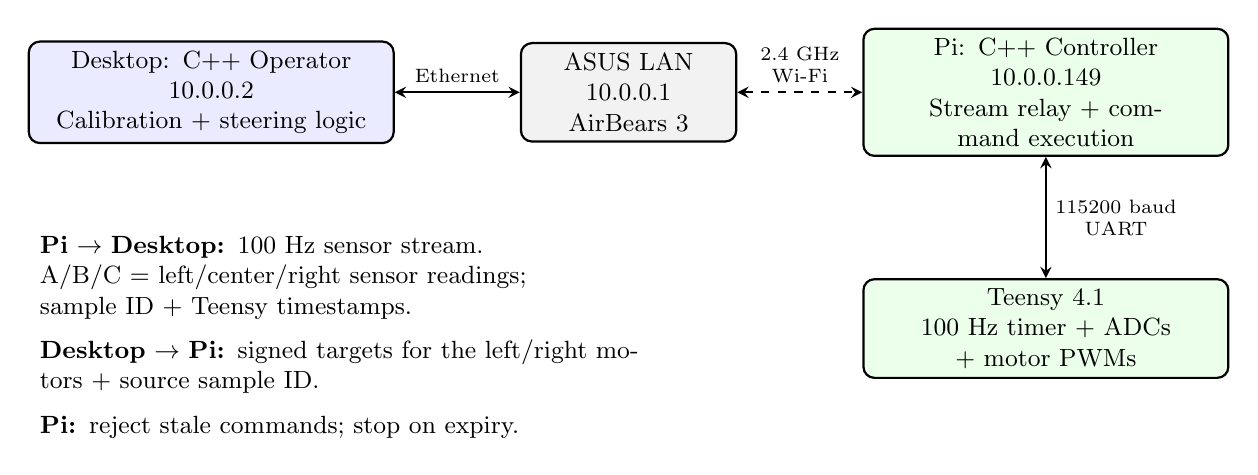
\begin{tikzpicture}[font=\small,>=stealth,
 block/.style={draw,thick,rounded corners,align=center,text width=4.4cm,minimum height=1.25cm},
 link/.style={<->,thick}, note/.style={font=\scriptsize,align=center,fill=white,inner sep=3pt}]
\node[block,fill=blue!8] (desktop) at (0,0) {Desktop: C++ Operator\\10.0.0.2\\Calibration + steering logic};
\node[block,fill=gray!10,text width=2.5cm] (asus) at (5.3,0) {ASUS LAN\\10.0.0.1\\AirBears 3};
\node[block,fill=green!8] (pi) at (10.6,0) {Pi: C++ Controller\\10.0.0.149\\Stream relay + command execution};
\node[block,fill=green!8] (teensy) at (10.6,-3.0) {Teensy 4.1\\100 Hz timer + ADCs + motor PWMs};
\draw[link] (desktop) -- node[note,above] {Ethernet} (asus);
\draw[link,dashed] (asus) -- node[note,above] {2.4 GHz\\Wi-Fi} (pi);
\draw[link] (pi) -- node[note,right] {115200 baud\\UART} (teensy);
\node[align=left,text width=7.9cm,anchor=north west] at (-2.3,-1.7) {\textbf{Pi $\to$ Desktop:} 100 Hz sensor stream.\\A/B/C = left/center/right sensor readings;\\sample ID + Teensy timestamps.\\[5pt]\textbf{Desktop $\to$ Pi:} signed targets for the left/right motors + source sample ID.\\[5pt]\textbf{Pi:} reject stale commands; stop on expiry.};
\end{tikzpicture}
}
\captionof{figure}{Network connectivity and distribution of control tasks.}
\label{fig:summary-network}
\end{center}
\vspace{-6pt}
\begin{center}
\resizebox{0.70\linewidth}{!}{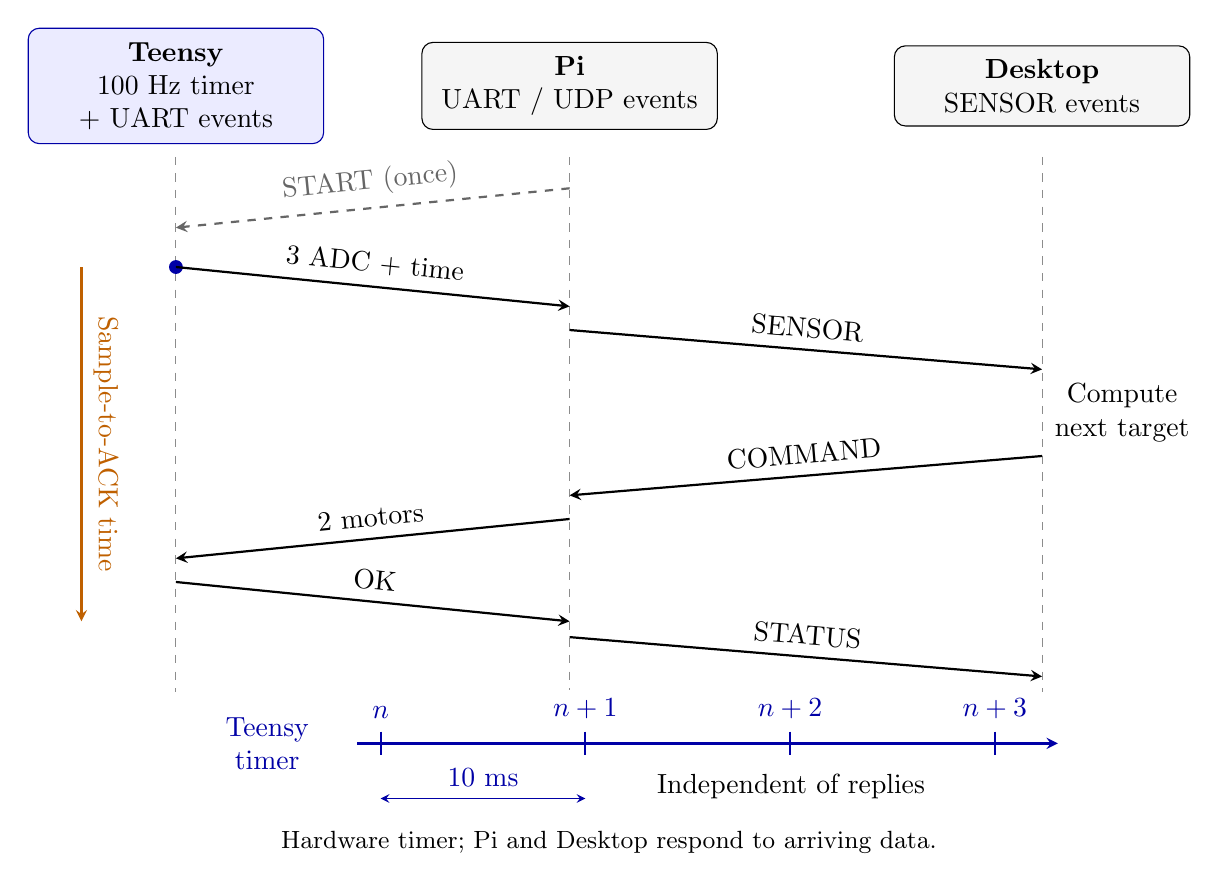
\begin{tikzpicture}[font=\normalsize,>=stealth,
 note/.style={font=\normalsize,fill=white,align=center,inner sep=3pt},
 arrowlabel/.style={font=\normalsize,sloped,above=3pt,inner sep=1pt},
 device/.style={draw,rounded corners,align=center,text width=3.4cm,inner sep=5pt},
 msg/.style={->,thick}]
\node[device,draw=blue!65!black,fill=blue!8] at (0,.5) {\textbf{Teensy}\\100 Hz timer\\+ UART events};
\node[device,fill=gray!8] at (5,.5) {\textbf{Pi}\\UART / UDP events};
\node[device,fill=gray!8] at (11,.5) {\textbf{Desktop}\\SENSOR events};
\foreach \x in {0,5,11} \draw[dashed,black!45] (\x,-.4) -- (\x,-7.2);
\fill[blue!65!black] (0,-1.8) circle (2.5pt);
\draw[msg,dashed,black!60] (5,-.8) -- node[arrowlabel] {START (once)} (0,-1.3);
\draw[msg] (0,-1.8) -- node[arrowlabel] {3 ADC + time} (5,-2.3);
\draw[msg] (5,-2.6) -- node[arrowlabel] {SENSOR} (11,-3.1);
\node[note,anchor=west] at (11.05,-3.65) {Compute\\next target};
\draw[msg] (11,-4.2) -- node[arrowlabel] {COMMAND} (5,-4.7);
\draw[msg] (5,-5.0) -- node[arrowlabel] {2 motors} (0,-5.5);
\draw[msg] (0,-5.8) -- node[arrowlabel] {OK} (5,-6.3);
\draw[msg] (5,-6.5) -- node[arrowlabel] {STATUS} (11,-7.0);
\draw[->,thick,orange!75!black] (-1.2,-1.8) -- node[arrowlabel] {Sample-to-ACK time} (-1.2,-6.3);
\node[note,text=blue!65!black,anchor=east] at (1.8,-7.85) {Teensy\\timer};
\draw[->,thick,blue!65!black] (2.3,-7.85) -- (11.2,-7.85);
\foreach \x/\n in {2.6/n,5.2/{n+1},7.8/{n+2},10.4/{n+3}} {
  \draw[thick,blue!65!black] (\x,-7.7) -- (\x,-8.0);
  \node[note,above,text=blue!65!black] at (\x,-7.65) {$\n$};
}
\draw[<->,blue!65!black] (2.6,-8.55) -- node[arrowlabel] {10 ms} (5.2,-8.55);
\node[note,anchor=west] at (6,-8.4) {Independent of replies};
\node[note,font=\small,anchor=north] at (5.5,-8.85) {Hardware timer; Pi and Desktop respond to arriving data.};
\end{tikzpicture}
}
\captionof{figure}{One control cycle.
Time flows downward. The sample-to-ACK interval includes the acknowledgement
back to Pi; the video's full round trip ends earlier, at Teensy target receipt.}
\label{fig:summary-step}
\end{center}
\clearpage
\begin{center}
{\Large\bfseries Robot and Remote-Control Demonstration}
\end{center}
\begin{center}
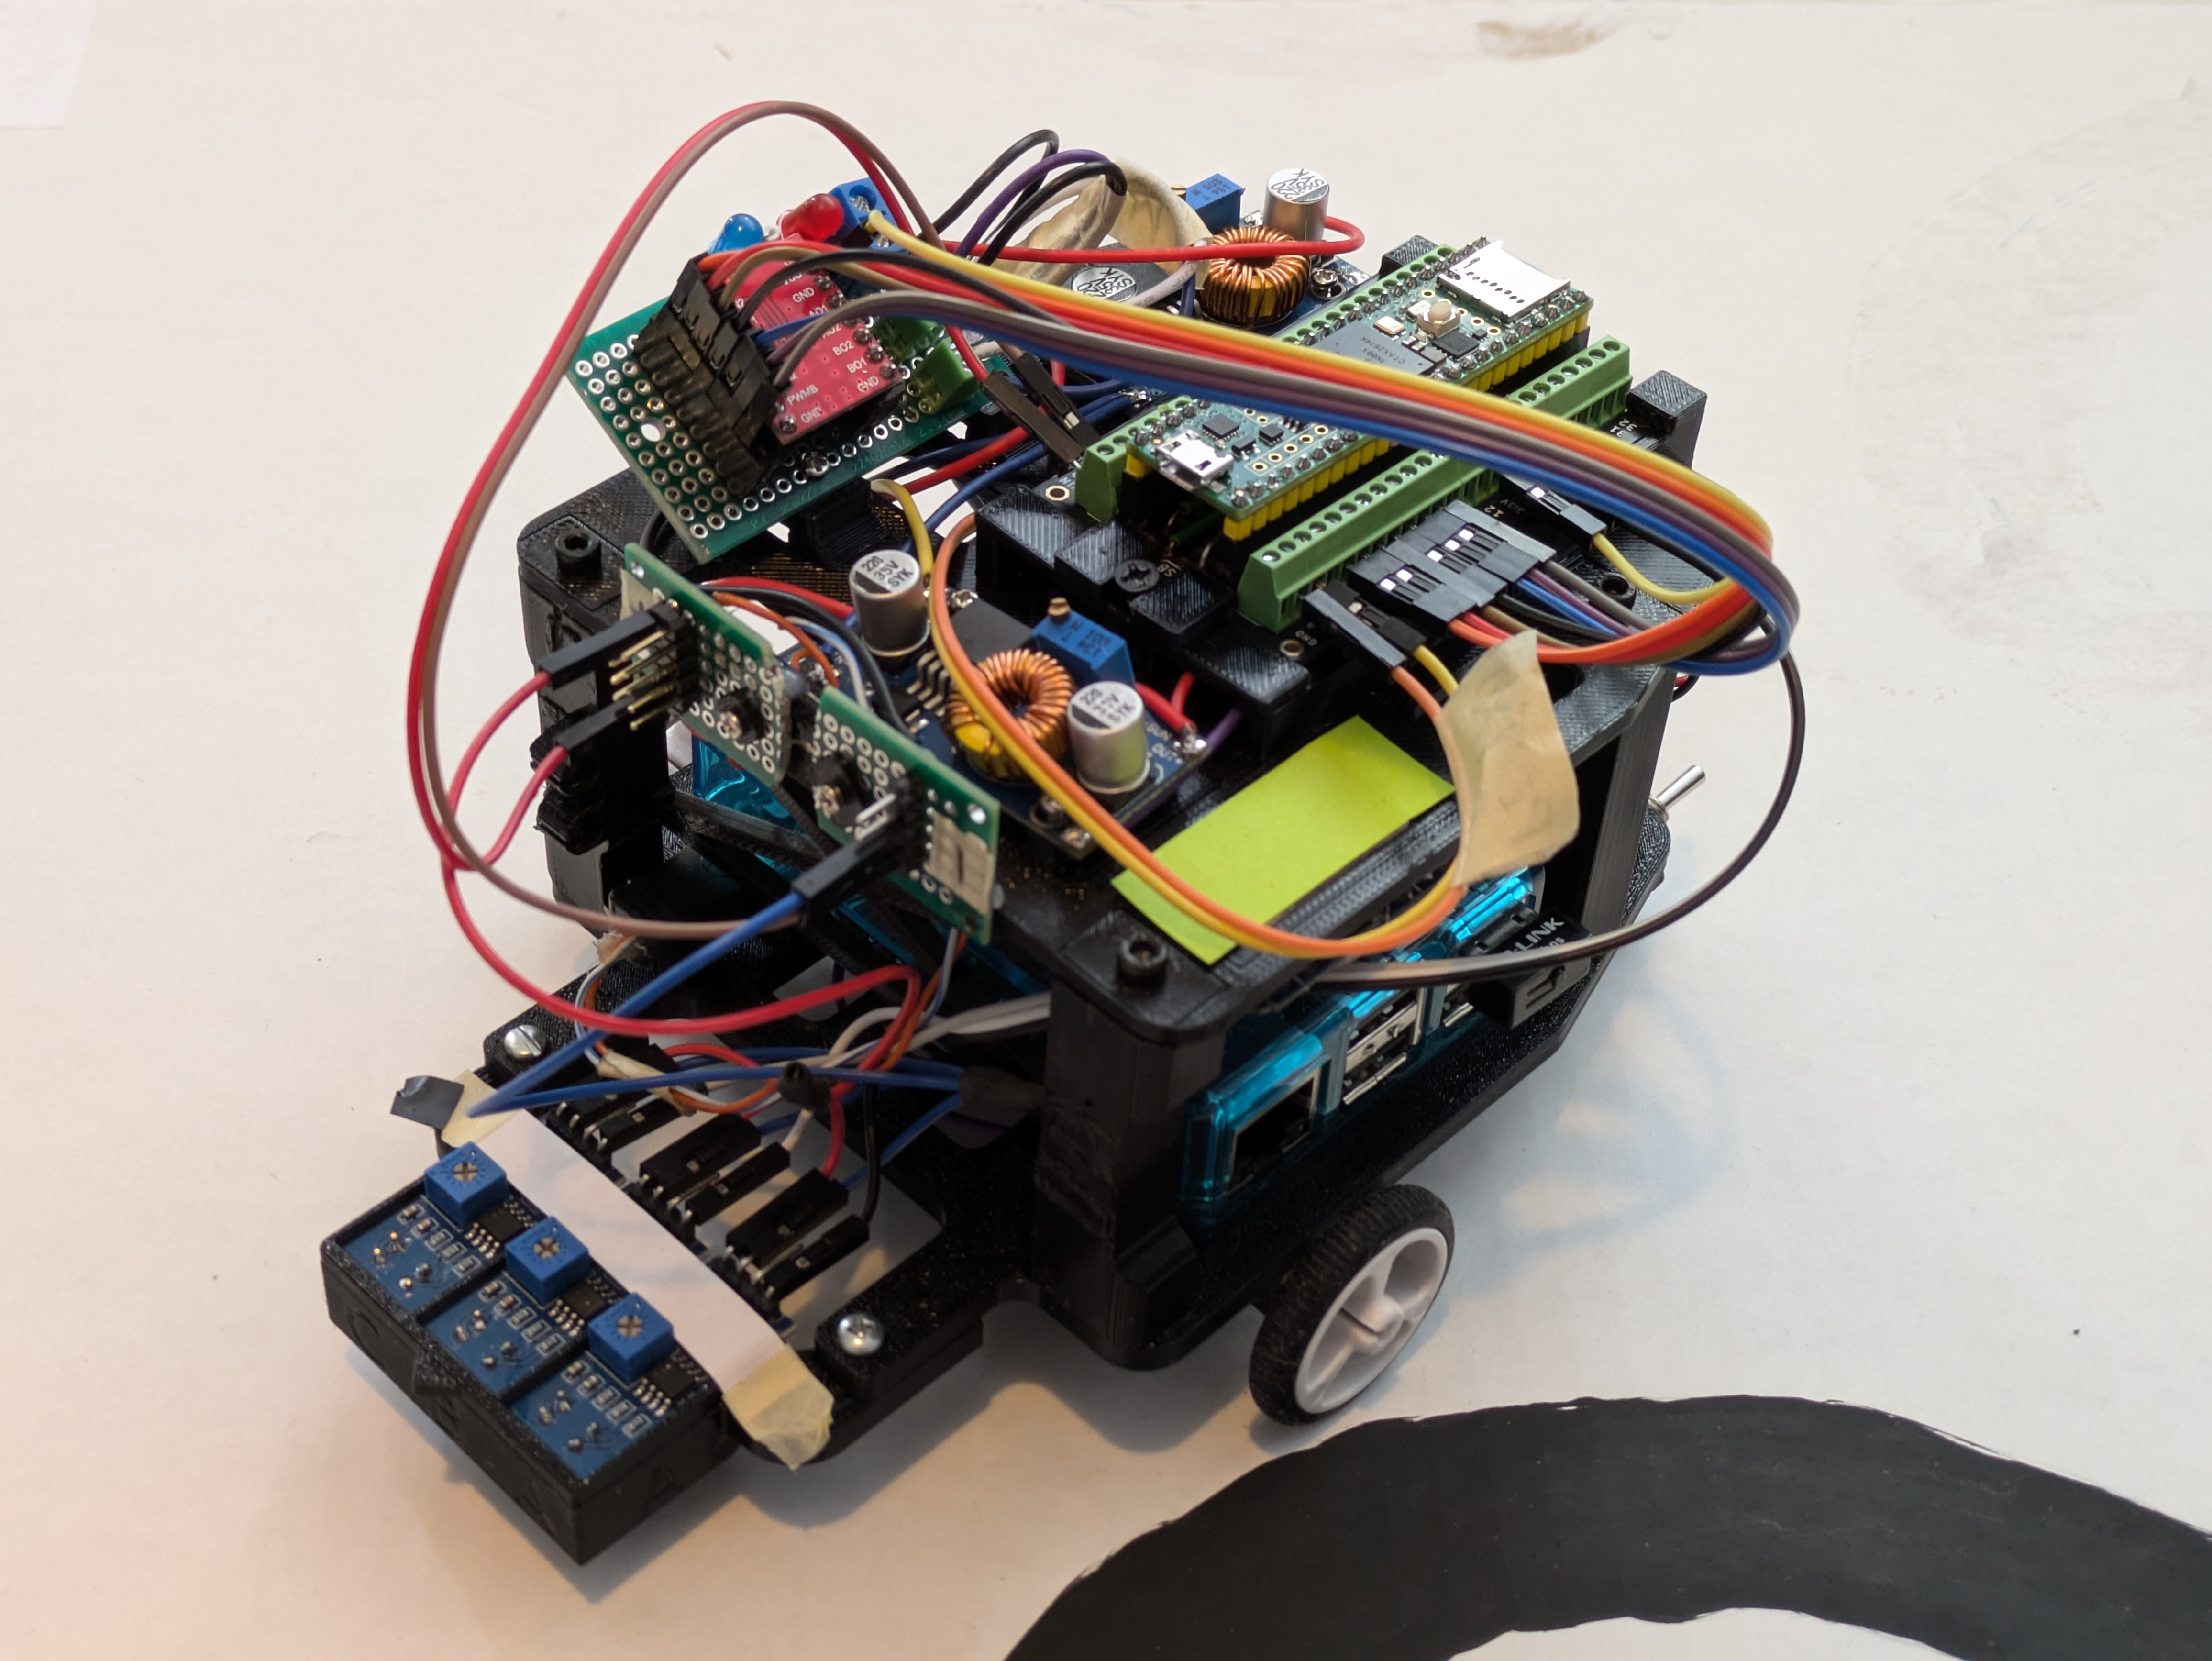
\includegraphics[width=0.82\linewidth,height=0.43\textheight,keepaspectratio]{line_follower_summary_figs/robot_photo.jpg}
\captionof{figure}{The assembled robot, with its front three-sensor head,
two driven wheels and stacked processing, motor-driver and power electronics.}
\label{fig:summary-photo}
\end{center}
\vfill
\begin{center}
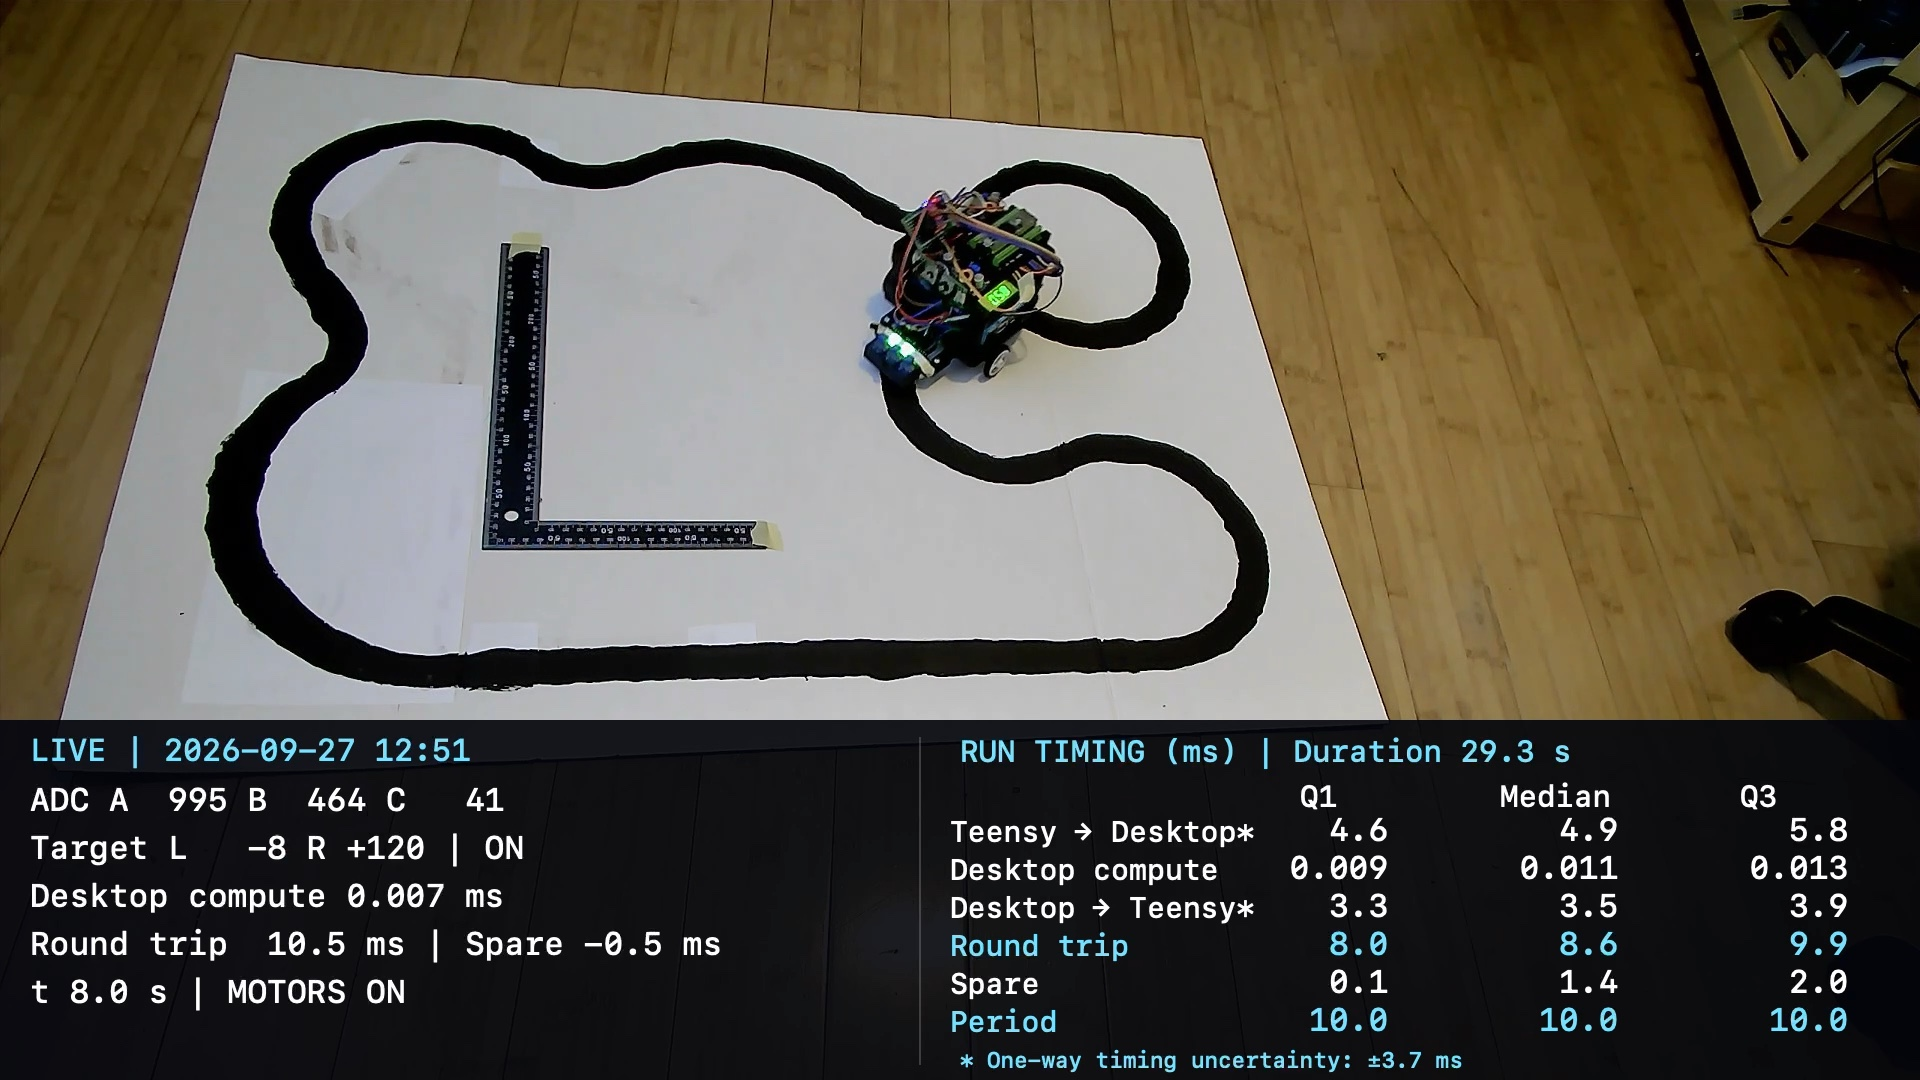
\includegraphics[width=\linewidth]{line_follower_summary_figs/frame_8.jpg}
\captionof{figure}{Video frame at $t=8.0$\,s. Live sensor readings and motor
targets appear at left; the table at right summarizes timing over the full
recorded run. Directional delays are estimates with the stated clock-alignment
uncertainty; full round trip is measured on Teensy's clock.}
\label{fig:summary-video}
\end{center}
\end{document}
